\subsection{Singulärwertverläufe als Werkzeug}
    Singulärwertverläufe sind das MIMO Analogon zu den SISO Bode-Plots. Der entscheidende Unterschied ist aber, dass man bei den SWV keine Information über die Phase hat und dass sie \textbf{worst-case Abschätzungen} sind im gegensatz zu effektiven Verstärkungen im Bode-Plot.
    
    Da bei Singulärwertverläufen die euklidische Norm des Eingans $= 1$ ist, \textbf{muss die euklidische Norm des Ausgangsvektors} $\mathbf{\in [\sigma_\textnormal{min},\sigma_\textnormal{max}]}$ \textbf{sein!}
    
    Die Singulärwertverläufe können für beliebige Übertragungsfunktionen ($S(s),\, T(s),\, L(s),\, Q(s)$) erstellt werden:
    \begin{align*}
        T(s) &= \big(I + P(s)\cdot C(s))\big)^{-1} \cdot P(s) \cdot C(s)\\
        S(s) &= \big(I + P(s)\cdot C(s))\big)^{-1}\\
        Q(s) &= I + P(s)\cdot C(s) \qquad\textnormal{(Return Difference)}
    \end{align*}
    
    Mit der Definition der Systemnorm
    \begin{equation*}
        \|G(s)\|_\infty = \max_\omega\bigg(\max_i \sigma_i\big(G(s)\big)\bigg),
    \end{equation*}
    hat dann z.B. die Sensitivität eine veranschulichende Interpretation: Die Systemnorm $\|S(s)\|_\infty$ ist die maximal zu erwartende/worst-case Verstärkung des Störsignals.
    
    \begin{figure}[H]
        \centering
        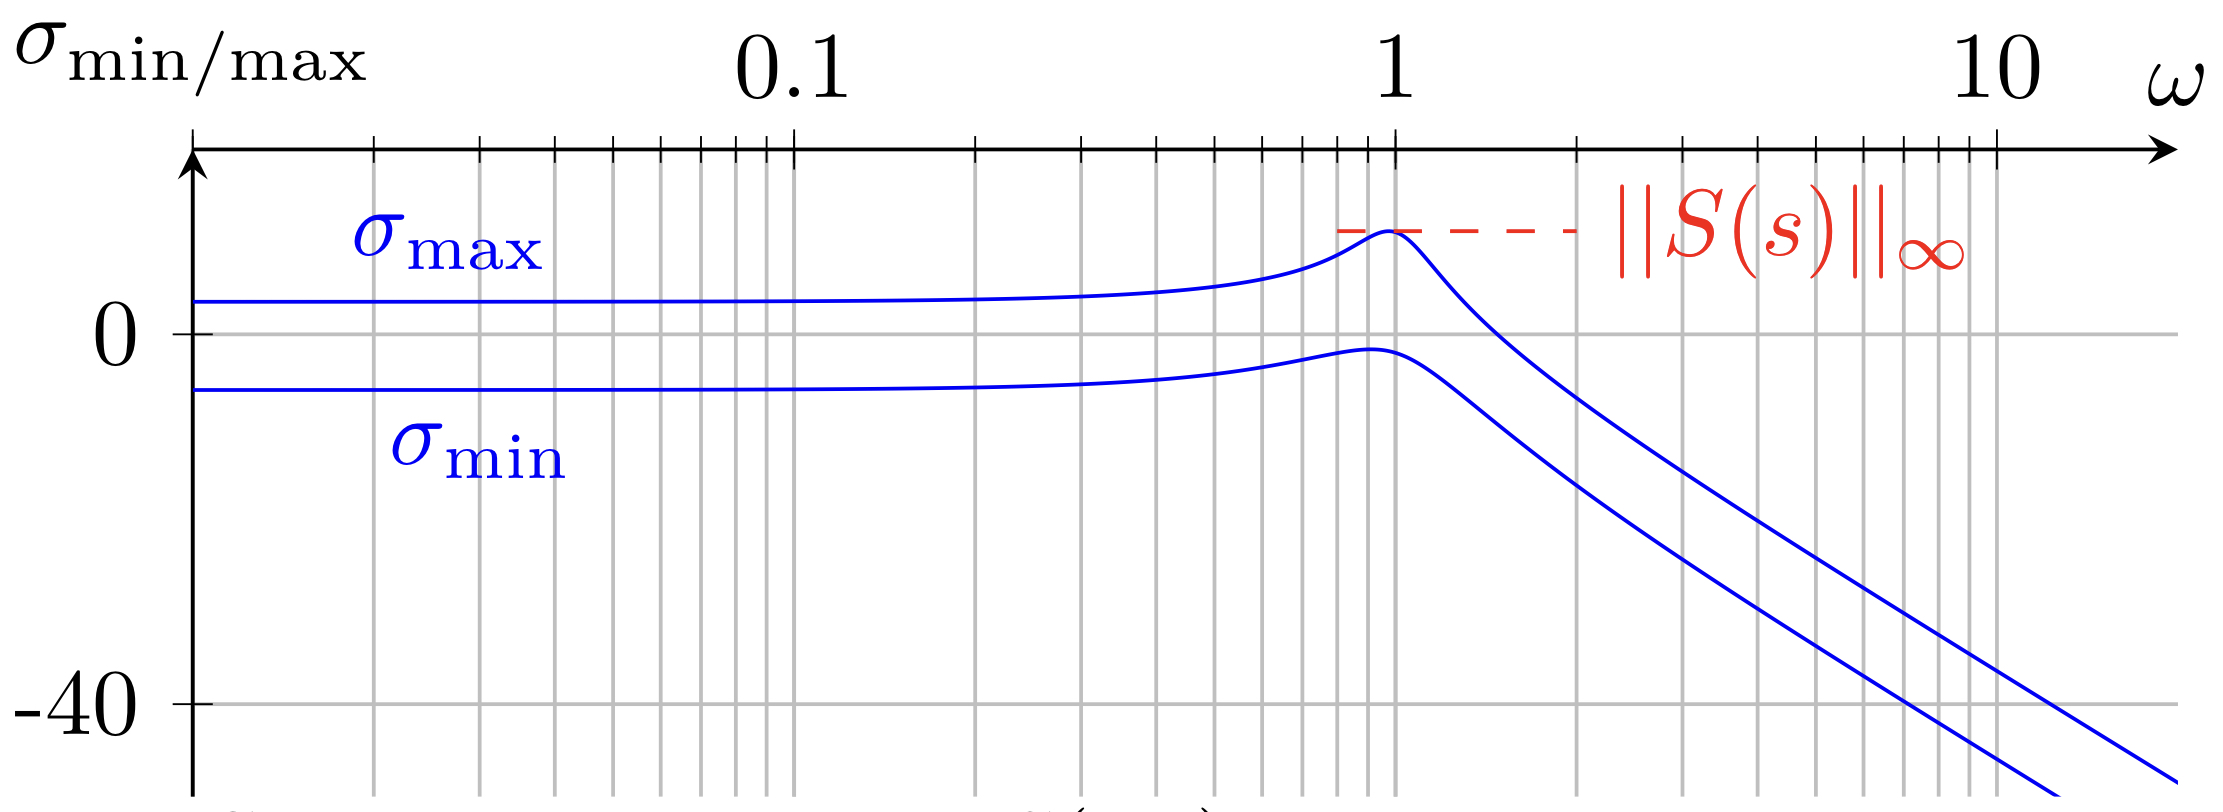
\includegraphics[width = 0.6\linewidth]{images/07/sysnorm.jpeg}
    \end{figure}
    Bei einer kleinen Systemnorm $\|S(s)\|_\infty$ weiss man, dass man eine gute Störungsunterdrückung hat.
    
    Die \textbf{Return Difference} gibt ein Mass für die Robustheit des Regelkreises:
    \begin{equation*}
        \colorboxed{red}{
        \mu_\textnormal{min} = \|Q\|_\infty
        }
    \end{equation*}